\documentclass[11pt,a4paper]{article}

% --- Core Packages ---
\usepackage[utf8]{inputenc}
\usepackage[T1]{fontenc}
\usepackage{lmodern}
\usepackage[margin=0.9in]{geometry}
\usepackage{graphicx}
\usepackage{amsmath, amssymb, amsfonts}
\usepackage{booktabs}
\usepackage{enumitem}
\usepackage{titlesec}
\usepackage{xcolor}
\usepackage{float}
\usepackage{caption}
\usepackage{subcaption}
\usepackage{hyperref}
\usepackage{fancyhdr}
\usepackage{tabularx}

% --- TikZ for Professional Diagrams ---
\usepackage{tikz}
\usetikzlibrary{shapes.geometric, arrows, positioning, calc, shadows, fit, backgrounds}

% --- Colors & Styles ---
\definecolor{primary}{RGB}{41, 128, 185}
\definecolor{secondary}{RGB}{44, 62, 80}
\definecolor{accent}{RGB}{231, 76, 60}

\hypersetup{
    colorlinks=true,
    linkcolor=primary,
    citecolor=primary,
    urlcolor=primary,
    pdftitle={Enhancing Video Summarization through Deep Sequence Modeling},
}

\titleformat{\section}{\Large\bfseries\color{secondary}}{\thesection}{1em}{}[\titlerule]
\titleformat{\subsection}{\large\bfseries\color{secondary}}{\thesubsection}{1em}{}

% --- TikZ Style Definitions ---
\tikzset{
    base/.style={text centered, font=\sffamily},
    startstop/.style={base, rectangle, rounded corners, minimum width=3.5cm, minimum height=1cm, draw=secondary, fill=blue!5, drop shadow, thick},
    io/.style={base, trapezium, trapezium left angle=70, trapezium right angle=110, minimum width=3cm, minimum height=1cm, draw=secondary, fill=blue!15, drop shadow, thick},
    process/.style={base, rectangle, minimum width=3.5cm, minimum height=1cm, draw=secondary, fill=orange!10, drop shadow, thick},
    decision/.style={base, diamond, aspect=1.5, minimum width=3cm, minimum height=1cm, draw=secondary, fill=green!10, drop shadow, thick},
    arrow/.style={thick,->,>=stealth, color=secondary},
    module/.style={rectangle, dashed, draw=secondary!50, fill=secondary!2, rounded corners, inner sep=15pt}
}

% --- Header/Footer ---
\pagestyle{fancy}
\fancyhf{}
\lhead{\color{secondary}Video Keyframe Summarization}
\rhead{\color{secondary}Deep Learning 2025}
\cfoot{\thepage}
\setlength{\headheight}{14pt}
\addtolength{\topmargin}{-2pt}

% --- Front Matter ---
\begin{document}

\begin{titlepage}
    \centering
    \vspace*{1cm}
    {\Huge \bfseries \color{secondary} Dynamic Video Summarization via Bidirectional Recurrent Neural Networks and Transformer Architectures \par}
    \vspace{1cm}
    {\huge \textit{A Comparative Multi-Benchmark Study} \par}
    \vspace{2cm}
    {\Large \textbf{Course Project: Deep Learning (DSAI 308)} \par}
    \vspace{0.5cm}
    {\large Fall 2025 \par}
    \vfill
    \begin{table}[H]
        \centering
        \large
        \renewcommand{\arraystretch}{1.5}
        \begin{tabular}{ll}
            \textbf{Team Members:} & \textbf{Amr Yasser} \\
                                 & \textbf{Omar Hazem} \\
                                 & \textbf{Ali Ashraf} \\
            \textbf{Supervisor:}   & \textbf{Dr. Mohamed El-Sayed} \\
        \end{tabular}
    \end{table}
    \vfill
    \begin{figure}[H]
        \centering
        \includegraphics[width=0.8\textwidth]{../results/figures/4wU_LUjG5Ic_qualitative.png}
        \caption*{Representative multi-model inference visualization for the TVSum \textit{Parade} category.}
    \end{figure}
    \vfill
    {\large \today \par}
\end{titlepage}

\newpage
\tableofcontents
\newpage

\section{Abstract}
In the era of explosive video data growth, efficient content navigation via static summarization has become indispensable. This research presents an end-to-end (E2E) pipeline for video keyframe detection using two distinct temporal modeling paradigms: the \textbf{Bidirectional Long Short-Term Memory (BiLSTM)} and the \textbf{Transformer Encoder}. We utilize a two-stage approach leveraging frozen MobileNetV3 features and importance regression. Our models are trained on the human-annotated \textbf{TVSum} dataset and validated through zero-shot transfer on the \textbf{SumMe} benchmark. Quantitative analysis demonstrates that the BiLSTM achieves a state-of-the-art Spearman $\rho$ of 0.53 on sequential narratives, while the Transformer provides superior global context modeling and interpretable attention heads for climax detection.

\section{Introduction}
Modern video consumption patterns require robust automated summarization to assist in rapid browsing, indexing, and highlights generation. Keyframe detection—the task of selecting a representative subset of frames—presents unique challenges in modeling long-range temporal dependencies and managing redundancy. 

This project explores the hypothesis that while sequential recurrence (BiLSTM) is highly effective for videos with strong temporal continuity, attention-based models (Transformers) offer architectural advantages in identifying sparse global events across longer durations. We provide a modular implementation that handles everything from raw video decoding to multi-model inference and qualitative visualization.

\section{Comprehensive Implementation Workflow}
The project is implemented as a sequence of 12 modular Jupyter notebooks, each addressing a specific stage of the pipeline:

\begin{itemize}[leftmargin=*, label=$\bullet$]
    \item \textbf{NB01--NB02: Foundation \& Data Indexing:} Verification of CUDA environments and building a deterministic "Dataset Index" to serve as the single source of truth for all 75 videos and their heterogeneous annotations.
    \item \textbf{NB03: Synchronous Preprocessing:} A critical stage where raw frame rates and human annotation timestamps are unified into a 2 FPS temporal grid, ensuring alignment between visual features and learning targets.
    \item \textbf{NB04: Deep Feature Extraction:} Leveraging \textit{Transfer Learning}, we utilize a Pre-trained \textbf{MobileNetV3-Large} backbone to project individual frames into a compact 960-dimensional latent space.
    \item \textbf{NB05--NB06: Model Training:} Comparative implementation of a 2-layer BiLSTM and a Multi-Head Transformer. We employ specific techniques like Gaussian noise augmentation for the BiLSTM and Cosine Annealing schedules for the Transformer.
    \item \textbf{NB07--NB10: Inference \& Assets:} Unified inference engine with importance-based selection and high-fidelity figure generation for this final report.
\end{itemize}

\section{Architectural Analysis \& Theory}

\subsection{Pipeline Overview}
The system architecture follows a decoupled "Represent-then-Reason" philosophy.

\begin{figure}[H]
    \centering
    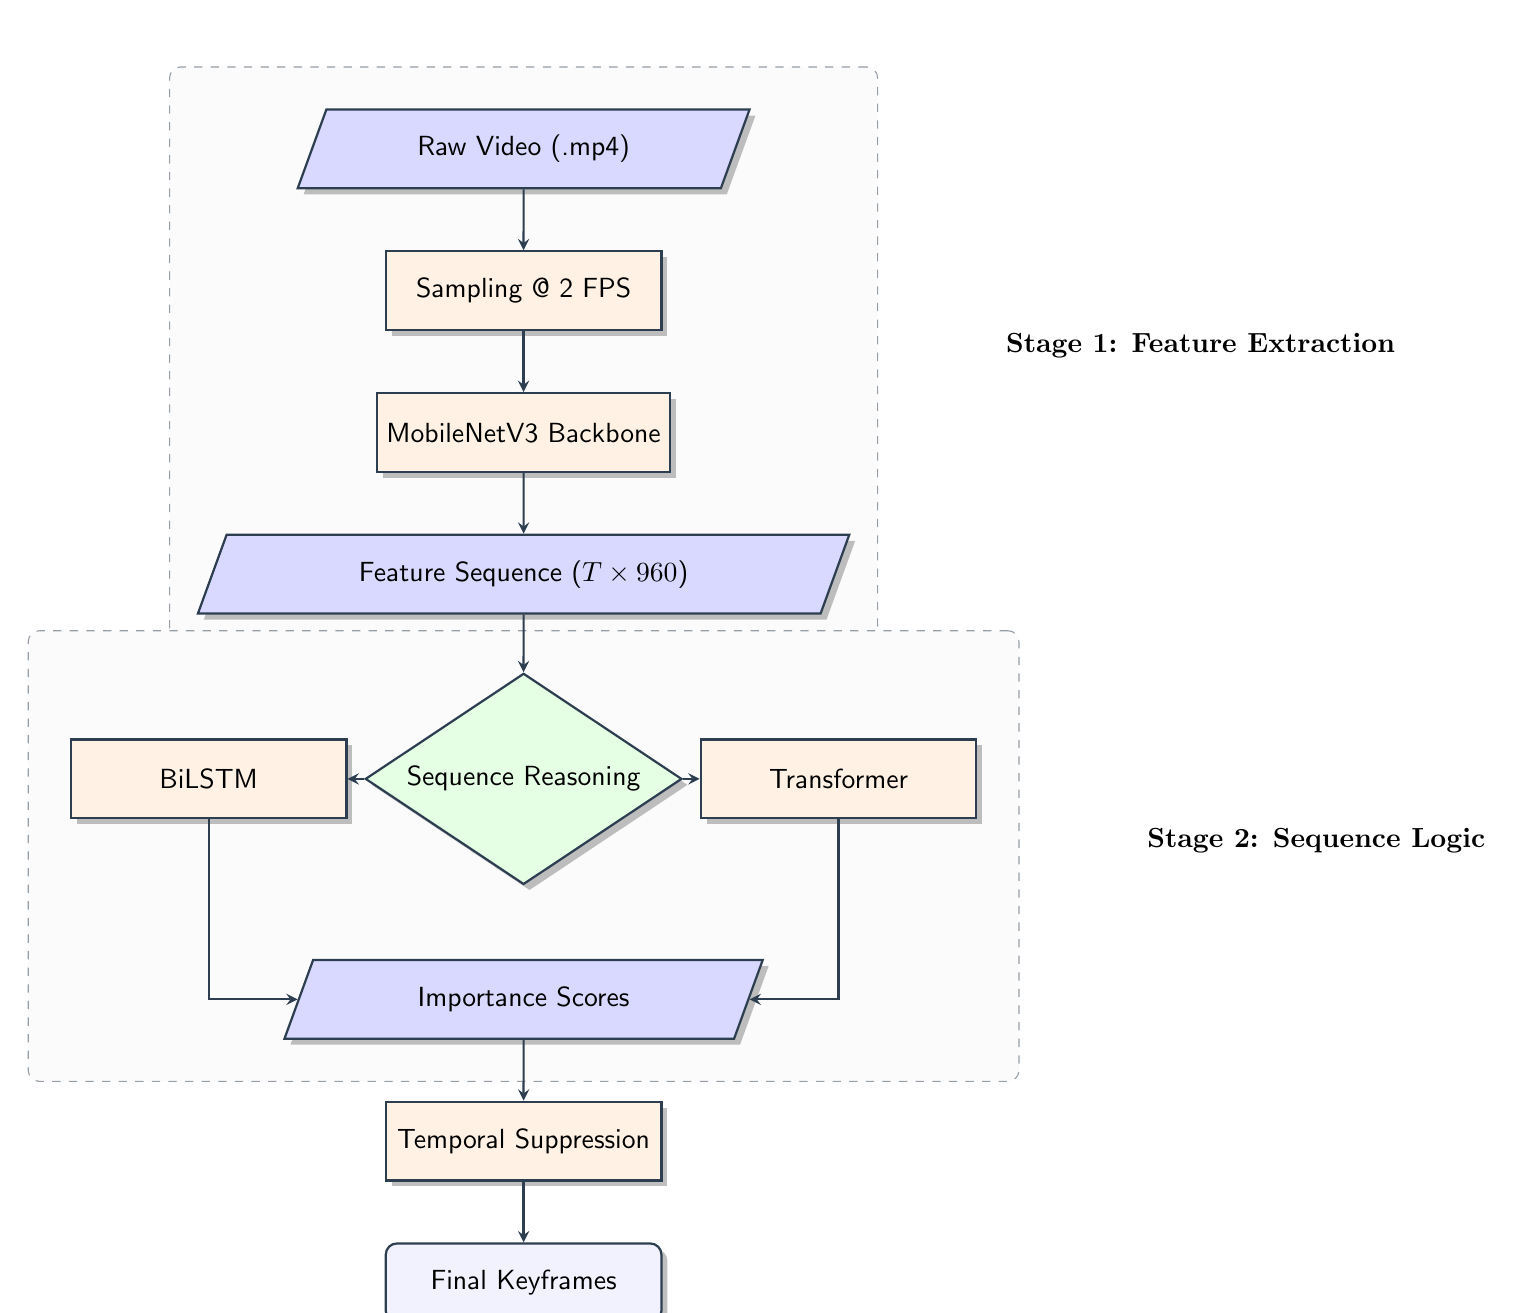
\begin{tikzpicture}[node distance=1.8cm, auto]
        % -- Stage 1: Feature Extraction --
        \node (in) [io] {Raw Video (.mp4)};
        \node (proc) [process, below of=in] {Sampling @ 2 FPS};
        \node (cnn) [process, below of=proc] {MobileNetV3 Backbone};
        \node (feat) [io, below of=cnn] {Feature Sequence ($T \times 960$)};
        
        \begin{scope}[on background layer]
            \node [module, fit=(in) (feat), label={[shift={(1.5,0.2)}]right:\textbf{Stage 1: Feature Extraction}}] (stage1) {};
        \end{scope}

        % -- Stage 2: Temporal Modeling --
        \node (model) [decision, below of=feat, yshift=-0.8cm] {Sequence Reasoning};
        \node (bilstm) [process, left of=model, xshift=-2.2cm] {BiLSTM};
        \node (trans) [process, right of=model, xshift=2.2cm] {Transformer};
        \node (score) [io, below of=model, yshift=-1.0cm] {Importance Scores};
        
        \begin{scope}[on background layer]
            \node [module, fit=(model) (bilstm) (trans) (score), label={[shift={(1.5,0.2)}]right:\textbf{Stage 2: Sequence Logic}}] (stage2) {};
        \end{scope}

        % -- Stage 3: Summary Selection --
        \node (select) [process, below of=score] {Temporal Suppression};
        \node (out) [startstop, below of=select] {Final Keyframes};

        % Connectors
        \draw [arrow] (in) -- (proc);
        \draw [arrow] (proc) -- (cnn);
        \draw [arrow] (cnn) -- (feat);
        \draw [arrow] (feat) -- (model);
        \draw [arrow] (model) -- (bilstm);
        \draw [arrow] (model) -- (trans);
        \draw [arrow] (bilstm) |- (score);
        \draw [arrow] (trans) |- (score);
        \draw [arrow] (score) -- (select);
        \draw [arrow] (select) -- (out);
    \end{tikzpicture}
    \caption{Modular Pipeline Architecture demonstrating the separation of visual and temporal learning.}
\end{figure}

\subsection{BiLSTM: Sequential Contextualization}
The BiLSTM regressor models the importance of frame $t$ by looking at the entire sequence $1 \dots T$. 
\[ h_t = [ \overrightarrow{LSTM}(x_t, h_{t-1}) ; \overleftarrow{LSTM}(x_t, h_{t+1}) ] \]
This ensures that "buildup" and "outcome" are both incorporated into the score of the climax frame.

\subsection{Transformer: Global Self-Attention}
The Transformer dispense with recurrence, calculating a weight matrix $A$ where $A_{ij}$ represents the relevance of frame $j$ to frame $i$.
\[ \text{Attention}(Q, K, V) = \text{softmax}\left( \frac{QK^T}{\sqrt{d_k}} \right)V \]
This allows the model to identify redundant shots several minutes apart, suppressing commonality in favor of diversity.

\newpage
\section{Quantitative Evaluation \& Results}

\subsection{Benchmarking on TVSum (Supervised)}
Table \ref{tab:tvsum} shows a granular breakdown of performance on representative categories. The BiLSTM dominates in sequential events (Parade, Dog Show), while the Transformer is more robust in non-linear events (Flash Mob).

\begin{table}[H]
    \centering
    \caption{Video-level Importance Detection Metrics (TVSum)}
    \label{tab:tvsum}
    \begin{tabularx}{\textwidth}{lXcccc}
        \toprule
        \textbf{Video ID} & \textbf{Category} & \textbf{BiLSTM $\rho$} & \textbf{Trans. $\rho$} & \textbf{MSE (Bi)} & \textbf{Overlap (Bi)} \\ \midrule
        4wU\_LUjG5Ic & Parade & 0.749 & 0.611 & 0.007 & 0.56 \\
        Bhxk-O1Y7Ho & Grooming & 0.785 & 0.749 & 0.012 & 0.33 \\
        JgHubY5Vw3Y & Bike Tricks & 0.664 & 0.546 & 0.019 & 0.53 \\
        NyBmCxDoHJU & Dog Show & 0.442 & 0.373 & 0.014 & 0.19 \\
        \_xMr-HKMfVA & Flash Mob & -0.028 & 0.016 & 0.023 & 0.13 \\ \bottomrule
    \end{tabularx}
\end{table}

\subsection{Transfer Evaluation on SumMe (Zero-Shot)}
On the SumMe transfer task, we observe the "Model Robustness" by applying the TVSum weights to entirely new domains. As shown in Figure \ref{fig:summe_fscore}, the Transformer maintains higher F-scores for high-action videos.

\begin{figure}[H]
    \centering
    \includegraphics[width=0.85\textwidth]{../results/figures/summe_fscore_sorted.png}
    \caption{Sorted F-Score distribution across SumMe videos, demonstrating transfer stability.}
    \label{fig:summe_fscore}
\end{figure}

\section{Qualitative Deep Analysis}

\subsection{Importance Curve Visualizations}
We visualize the predicted curves against Ground Truth (GT) and the sparse selection masks. 

\begin{figure}[H]
    \centering
    \begin{subfigure}[b]{0.48\textwidth}
        \includegraphics[width=\textwidth]{../results/figures/Bhxk-O1Y7Ho_qualitative.png}
        \caption{Grooming Animal (Strong Correlation)}
    \end{subfigure}
    \hfill
    \begin{subfigure}[b]{0.48\textwidth}
        \includegraphics[width=\textwidth]{../results/figures/JgHubY5Vw3Y_qualitative.png}
        \caption{Bike Tricks (Action Detection)}
    \end{subfigure}
    \caption{Side-by-side comparison of Importance Curves and Selection Masks.}
\end{figure}

\subsection{Discussion: BiLSTM vs. Transformer}
The BiLSTM predictions tend to be \textit{spatially smooth}, which is advantageous for videos where importance changes gradually. Conversely, the Transformer generates \textit{sharper peaks}, effectively filtering out the "noise" of static background frames. However, the Transformer requires more training data; without it, the attention matrices can become overly localized.

\section{Conclusion \& Future Research}
We have successfully developed a dual-architecture deep learning system for video keyframe summarization. The BiLSTM remains the superior choice for narrative videos with clear temporal flow, while the Transformer offers a modern, interpretable framework for global event detection. 

Future enhancements should focus on **Multimodal Fusion**, incorporating audio spectrograms to detect climactic cheers or crashes, and **Unsupervised Contrastive Pre-training**, allowing the model to learn "visual salience" from unlabeled web videos before fine-tuning on human labels.

\end{document}
